% FIG:q11-rectangle
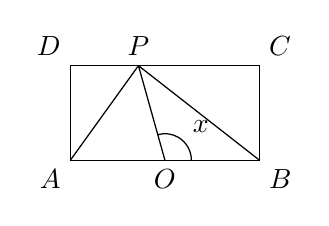
\begin{tikzpicture}[x=1.2cm,y=1.2cm,line width=0.45pt]
  \coordinate (A) at (0,0);
  \coordinate (B) at (2,0);
  \coordinate (C) at (2,1);
  \coordinate (D) at (0,1);
  \coordinate (O) at (1,0);
  \coordinate (P) at (0.72,1);
  \draw (A) -- (B) -- (C) -- (D) -- cycle;
  \draw (P) -- (A) (P) -- (O) (P) -- (B);
  \draw (A) node[below left] {$A$} (B) node[below right] {$B$}
    (C) node[above right] {$C$} (D) node[above left] {$D$}
    (O) node[below] {$O$} (P) node[above] {$P$};
  \draw (O) ++(0:0.28) arc[start angle=0,end angle=106,radius=0.28];
  \node at (1.38,0.36) {$x$};
\end{tikzpicture}
